% Provenance (never printed): see sources/outline_sources.md (Year 1: crystal
% chemistry of minerals, silicates, solid solutions, mineral formulas, the main
% rock-forming minerals). Olivine curves in figdata/bachelor-1/solid_solution.py;
% the olivine analysis of the problem is invented (Fo about 82); exercise and
% problem values in the Book 3 scratch calculator calc/ch07.py.
\chapter{Gesteentevormende mineralen}\label{ch:b1:rock-forming-minerals}

Een granieten aanrechtblad toont drie of vier soorten korrels: glazig grijze kwarts, roze of witte
\omterm{def:b1:rock-forming-minerals:groups}{veldspaat}, plaatjes van zwarte \omterm{def:b1:rock-forming-minerals:groups}{mica}. Strandzand is bijna geheel kwarts. De kleine groene kristallen die in een
basalt zijn verspreid, zijn \omterm{def:b1:rock-forming-minerals:groups}{olivijn}, en hetzelfde \omterm{def:b1:rock-forming-minerals:mineral}{mineraal}, met een iets andere samenstelling, vormt het grootste
deel van de bovenste mantel. Een handvol mineralen bouwt bijna elk gesteente, en vrijwel allemaal zijn het
silicaten: zuurstof en silicium, de twee meest voorkomende elementen van de korst, verbonden tot tetraëders die
op een paar eenvoudige manieren aan elkaar schakelen. Dit hoofdstuk legt uit hoe de koppeling de formule en de habitus
van een silicaat bepaalt, hoe het ene element in een kristal het andere vervangt zodat een \omterm{def:b1:rock-forming-minerals:mineral}{mineraal} een reeks
samenstellingen is in plaats van één, hoe een chemische analyse een formule wordt, en wat de belangrijkste
gesteentevormende mineralen zijn. Het eindigt met een \omterm{def:b1:rock-forming-minerals:groups}{olivijn} uit een basalt, geanalyseerd, herberekend en
gewogen.

\begin{recall}
Een kristal is een vaste stof waarvan de atomen zich op een rooster herhalen; de eenheidscel is de kleinste doos
die zich herhaalt, en het coördinatiegetal van een ion telt zijn naaste buren van tegengestelde lading (scheikunde,
eerste jaar universiteit). Ionstralen hangen af van de lading en van de coördinatie. Een \omterm{def:b1:rock-forming-minerals:mineral}{mineraal} wordt in de hand
herkend aan zijn habitus, splijting, hardheid en glans (Boek 2, klas 11). De hoeveelheid stof wordt geteld in mol, en
een molaire massa is de massa van één mol (scheikunde).
\end{recall}

\section{Wat een mineraal is}

\begin{definition}[Mineraal]\label{def:b1:rock-forming-minerals:mineral}
Een \emph{mineraal}\index{mineraal} is een natuurlijk voorkomende vaste stof met een bepaalde kristalstructuur en een
chemische samenstelling die vast is of binnen bepaalde grenzen varieert. Bijna alle mineralen zijn anorganisch.
\end{definition}

Een gesteente is daarentegen een aggregaat van korrels van één of meer mineralen (of van glas): graniet bestaat uit
kwarts, veldspaten en \omterm{def:b1:rock-forming-minerals:groups}{mica}; kalksteen bestaat meestal uit calciet. De twee helften van de definitie zijn onafhankelijk.
Vensterglas heeft de samenstelling van een silicaat maar geen kristalstructuur: het is geen \omterm{def:b1:rock-forming-minerals:mineral}{mineraal}, net zo min als
het glas van een snel afgekoelde lava. Omgekeerd kan dezelfde samenstelling in verschillende structuren kristalliseren,
en elke structuur is een ander \omterm{def:b1:rock-forming-minerals:mineral}{mineraal}.

\begin{definition}[Polymorf]\label{def:b1:rock-forming-minerals:polymorph}
Twee mineralen zijn \emph{polymorfen}\index{polymorf} van elkaar wanneer zij dezelfde chemische samenstelling hebben
maar verschillende kristalstructuren.
\end{definition}

Koolstof kristalliseert als grafiet, een stapel vellen van zeshoeken met een dichtheid van \qty{2.16}{g.cm^{-3}}, en als
diamant, een raamwerk waarin elk atoom vier buren heeft, met een dichtheid van \qty{3.51}{g.cm^{-3}}. Calciumcarbonaat is
calciet (\qty{2.71}{g.cm^{-3}}) of aragoniet (\qty{2.93}{g.cm^{-3}}); siliciumdioxide is kwarts (\qty{2.65}{g.cm^{-3}})
of coesiet (\qty{2.93}{g.cm^{-3}}); \ce{Al2SiO5} is kyaniet (\qty{3.61}{g.cm^{-3}}), andalusiet (\qty{3.15}{g.cm^{-3}})
of sillimaniet (\qty{3.24}{g.cm^{-3}}).
% ledger: webmineral:polymorphs, hom:calcite, hom:quartz
In elk paar is de dichtere \omterm{def:b1:rock-forming-minerals:polymorph}{polymorf} de vorm die bij hogere druk ontstaat: bij een gegeven temperatuur bevordert
drukverhoging de toestand van het kleinere volume (scheikunde, de verschuiving van een evenwicht). Diamant in een
kimberliet en coesiet in een gesteente dat door een meteoriet is getroffen, leggen daarom drukken vast die alleen diep in
de mantel of bij een inslag voorkomen. De drie \ce{Al2SiO5}-polymorfen, waarvan de stabiliteitsvelden het druk--temperatuurvlak
onder elkaar verdelen, worden gebruikt om de omstandigheden van metamorfose af te lezen (tweede jaar universiteit).

\section{Het silicaattetraëder en zijn koppelingen}

In elk gewoon silicaat zit elk siliciumatoom in het midden van vier zuurstofatomen, geplaatst op de hoeken van een regelmatig
tetraëder: de \ce{SiO4}-eenheid uit de scheikunde. Het siliciumion is klein (\qty{0.26}{\angstrom} in viervoudige coördinatie)
en het oxide-ion groot, zodat vier zuurstoffen eromheen passen en niet meer; de silicium--zuurstofbinding is sterk en
gedeeltelijk covalent. Een geïsoleerde eenheid draagt een lading $4 - 4\times2 = -4$.
% ledger: shannon:radii
De tetraëders kunnen op zichzelf staan, hun lading in balans gebracht door metaalkationen ertussen, of hoeken delen: een
zuurstof die tot twee tetraëders behoort, is een \emph{brugzuurstof}. Twee tetraëders delen nooit een
rand of een vlak, want dan zouden twee siliciumatomen te dicht bij elkaar komen. Silicaten worden ingedeeld naar het aantal
hoeken dat elk tetraëder deelt (\cref{def:b1:rock-forming-minerals:silicate-classes}).

\begin{omfigure}
\tikzset{
  tup/.pic={\filldraw[fill=omLithLime, draw=black, line join=round] (0,0) -- (1,0) -- (0.5,0.866) -- cycle;
            \fill[omThm] (0.5,0.2887) circle (0.11);},
  tdn/.pic={\filldraw[fill=omLithLime, draw=black, line join=round] (0,0) -- (1,0) -- (0.5,-0.866) -- cycle;
            \fill[omThm] (0.5,-0.2887) circle (0.11);},
  linkpanel/.style={x=0.45cm, y=0.45cm, baseline=(current bounding box.south)}}
\setlength{\tabcolsep}{4pt}
\begin{tabular}{cccc}
% (a) the tetrahedron in perspective
\begin{tikzpicture}[linkpanel]
  \useasboundingbox (-1.2,-1.0) rectangle (6.0,4.4);
  \coordinate (T) at (2.2,3.7); \coordinate (L) at (0.3,0.5); \coordinate (R) at (4.1,0.1);
  \coordinate (B) at (3.3,2.1); \coordinate (C) at (2.475,1.6);
  \draw[densely dashed, gray] (L) -- (B) -- (R) (B) -- (T);
  \shade[ball color=omLithShale] (B) circle (0.42);
  \draw[gray] (C) -- (T) (C) -- (L) (C) -- (R) (C) -- (B);
  \shade[ball color=omThm!70] (C) circle (0.24);
  \draw[thick, line join=round] (T) -- (L) -- (R) -- cycle;
  \foreach \p in {T,L,R} \shade[ball color=omLithShale] (\p) circle (0.42);
  \node[right] at (4.5,0.1) {\scriptsize O};
  \node[right] at (2.6,3.8) {\scriptsize O};
  \draw[omThm] (C) -- (4.6,2.2) node[right] {\scriptsize Si};
\end{tikzpicture} &
% (b) nesosilicate: isolated tetrahedra
\begin{tikzpicture}[linkpanel]
  \useasboundingbox (-1.2,-1.0) rectangle (6.0,4.4);
  \pic at (0,0.3) {tup}; \pic at (2.4,0.3) {tup}; \pic at (4.0,1.9) {tdn};
  \pic at (1.2,2.4) {tdn}; \pic at (3.0,2.8) {tup};
\end{tikzpicture} &
% (c) sorosilicate: pairs
\begin{tikzpicture}[linkpanel]
  \useasboundingbox (-1.2,-1.0) rectangle (6.0,4.4);
  \pic at (0,0.9) {tup}; \pic at (1,0.9) {tdn};
  \pic at (2.6,2.6) {tup}; \pic at (3.6,2.6) {tdn};
\end{tikzpicture} &
% (d) cyclosilicate: a ring of six
\begin{tikzpicture}[linkpanel]
  \useasboundingbox (-1.2,-1.0) rectangle (6.0,4.4);
  \begin{scope}[shift={(2.4,1.7)}]
  \foreach \t in {0,60,...,300} {
    \filldraw[fill=omLithLime, draw=black, line join=round] (\t-30:1) -- (\t+30:1) -- (\t:1.732) -- cycle;
    \fill[omThm] (\t:1.155) circle (0.11);}
  \end{scope}
\end{tikzpicture} \\
{\small (a) het \ce{SiO4}-tetraëder} & {\small (b) \omterm{def:b1:rock-forming-minerals:silicate-classes}{nesosilicaat}} & {\small (c) \omterm{def:b1:rock-forming-minerals:silicate-classes}{sorosilicaat}} & {\small (d) \omterm{def:b1:rock-forming-minerals:silicate-classes}{cyclosilicaat}} \\
 & {\scriptsize $s = 0$, \ce{SiO4}} & {\scriptsize $s = 1$, \ce{Si2O7}} & {\scriptsize $s = 2$, \ce{Si6O18}} \\[6pt]
% (e) single chain
\begin{tikzpicture}[linkpanel]
  \useasboundingbox (-0.6,-1.2) rectangle (7.6,4.6);
  \begin{scope}[shift={(0,1.5)}]
  \foreach \i in {0,...,3} \pic at (2*\i,0) {tup};
  \foreach \i in {0,...,2} \pic at (2*\i+1,0) {tdn};
  \end{scope}
\end{tikzpicture} &
% (f) double chain: two single chains joined through every other apex
\begin{tikzpicture}[linkpanel]
  \useasboundingbox (-0.6,-1.2) rectangle (7.6,4.6);
  \begin{scope}[shift={(0.5,0.4)}]
  \foreach \i in {0,...,3} {\pic at (2*\i,0) {tup}; \pic at (2*\i,1.732) {tdn};}
  \foreach \i in {0,...,2} {\pic at (2*\i+1,0) {tdn}; \pic at (2*\i+1,1.732) {tup};}
  \end{scope}
\end{tikzpicture} &
% (g) sheet
\begin{tikzpicture}[linkpanel]
  \useasboundingbox (-0.6,-1.2) rectangle (7.6,4.6);
  \foreach \j in {0,1,2} {
    \foreach \i in {0,1,2} {\pic at (2*\i+\j,1.732*\j) {tup};}
    \foreach \i in {0,1} {\pic at (2*\i+\j+1,1.732*\j) {tdn};}}
\end{tikzpicture} &
% (h) framework: a sheet whose apices point alternately up and down
\begin{tikzpicture}[linkpanel]
  \useasboundingbox (-0.6,-1.2) rectangle (7.6,4.6);
  \foreach \j in {0,1,2} {
    \foreach \i in {0,1,2} {\pic at (2*\i+\j,1.732*\j) {tup};}
    \foreach \i in {0,1} {\pic at (2*\i+\j+1,1.732*\j) {tdn};}}
  \foreach \j in {0,1,2} \foreach \i in {0,1} {
    \filldraw[fill=white, draw=omThm, thick] (2*\i+\j+1.5,1.732*\j-0.2887) circle (0.17);}
\end{tikzpicture} \\
{\small (e) enkelvoudige keten} & {\small (f) dubbele keten} & {\small (g) laag} & {\small (h) raamwerk} \\
{\scriptsize $s = 2$, \ce{SiO3}} & {\scriptsize $s = 2$ en $3$, \ce{Si4O11}} & {\scriptsize $s = 3$, \ce{Si2O5}} & {\scriptsize $s = 4$, \ce{SiO2}} \\
\end{tabular}
\medskip

{\small Het \ce{SiO4}-tetraëder (a) en de manieren waarop tetraëders aan elkaar schakelen, van boven gezien: elke driehoek
is de basis van een tetraëder, met drie zuurstoffen op de hoeken, de vierde erboven, de stip die het silicium aangeeft.
Hoeken die op elkaar liggen zijn gedeelde zuurstoffen; $s$ is het aantal hoeken dat elk tetraëder deelt. In het raamwerk (h)
zijn de top-zuurstoffen (open cirkels: naar beneden gericht; stippen: naar boven gericht) ook gedeeld, met de lagen
eronder en erboven.}
\end{omfigure}

\begin{definition}[De silicaatklassen]\label{def:b1:rock-forming-minerals:silicate-classes}
Silicaten worden ingedeeld naar hoe hun \ce{SiO4}-tetraëders aan elkaar schakelen. In een
\emph{nesosilicaat}\index{nesosilicaat} zijn de tetraëders geïsoleerd; in een \emph{sorosilicaat}\index{sorosilicaat}
zijn zij in paren verbonden door één gedeelde zuurstof; in een \emph{cyclosilicaat}\index{cyclosilicaat} vormen zij
gesloten ringen, elk met twee gedeelde hoeken; in een \emph{inosilicaat}\index{inosilicaat} vormen zij eindeloze ketens,
enkelvoudig (elk tetraëder deelt twee hoeken) of dubbel (twee enkelvoudige ketens naast elkaar, de helft van de
tetraëders deelt drie hoeken); in een \emph{fyllosilicaat}\index{fyllosilicaat} vormen zij eindeloze lagen, elk met drie
gedeelde hoeken; in een \emph{tectosilicaat}\index{tectosilicaat} vormen zij een driedimensionaal raamwerk, elk met alle
vier hoeken gedeeld.
\end{definition}

\begin{proposition}[De verhouding silicium tot zuurstof]\label{prop:b1:rock-forming-minerals:si-o}
Als elk \ce{SiO4}-tetraëder van een silicaat gemiddeld $s$ van zijn vier hoeken deelt met andere tetraëders, en elke
gedeelde zuurstof tot precies twee tetraëders behoort, dan bevat het silicaatnetwerk $4 - s/2$ zuurstoffen per silicium,
en draagt het een lading van $s - 4$ per silicium.
\end{proposition}

\begin{proof}
Tel de zuurstoffen tetraëder voor tetraëder. Een tetraëder met $s_i$ gedeelde hoeken bezit zijn $4 - s_i$ niet-gedeelde
zuurstoffen volledig en de helft van elk van zijn $s_i$ gedeelde, want elk wordt door het naburige tetraëder opnieuw geteld:
het levert $4 - s_i + s_i/2 = 4 - s_i/2$ zuurstoffen. Optellen over $N$ tetraëders en delen door $N$ geeft $4 - s/2$ zuurstoffen
per silicium, met $s$ het gemiddelde van de $s_i$. Elk silicium brengt een lading $+4$ en elke zuurstof $-2$, dus de lading per
silicium is $4 - 2(4 - s/2) = s - 4$.
\end{proof}

De stelling geeft meteen het anion van elke klasse. Geïsoleerde tetraëders ($s = 0$): \ce{SiO4^{4-}}. Paren ($s = 1$):
$4 - 1/2 = 7/2$, dat is \ce{Si2O7^{6-}}. Ringen en enkelvoudige ketens ($s = 2$): \ce{SiO3^{2-}}, geschreven als
\ce{Si6O18^{12-}} voor een ring van zes, \ce{Si2O6^{4-}} voor twee tetraëders van een keten. Dubbele ketens (de helft met
$s = 2$, de helft met $s = 3$, dus $s = 5/2$): $4 - 5/4 = 11/4$, \ce{Si4O11^{6-}}. Lagen ($s = 3$): \ce{Si2O5^{2-}}.
Raamwerken ($s = 4$): \ce{SiO2}, neutraal --- kwarts is een raamwerk van alleen silicium en zuurstof. Hoe meer de tetraëders
delen, hoe kleiner de lading die moet worden gecompenseerd en hoe minder metaalkationen er nodig zijn: \omterm{def:b1:rock-forming-minerals:groups}{olivijn} \ce{Mg2SiO4}
heeft twee metaalionen per silicium, een \omterm{def:b1:rock-forming-minerals:groups}{pyroxeen} zoals enstatiet \ce{Mg2Si2O6} één, kwarts geen.

De koppeling vormt ook het kristal. Een \omterm{def:b1:rock-forming-minerals:silicate-classes}{fyllosilicaat} splijt gemakkelijk tussen zijn lagen, waar de bindingen zwak zijn:
\omterm{def:b1:rock-forming-minerals:groups}{micas} splijten tot dunne buigzame plaatjes. Ketensilicaten splijten evenwijdig aan hun ketens, langs twee vlakken onder een hoek
die vastligt door hoe de ketens samenpakken: ongeveer \ang{87} en \ang{93} in pyroxenen, waarvan de ketens smal zijn, \ang{56} en
\ang{124} in amfibolen, waarvan de dubbele ketens breder zijn. De twee splijthoeken, gezien op een gebroken kristal of in een
\omterm{def:b1:field-lab-methods-1:thin-section}{dunne slijpplaat}, zijn de klassieke manier om de twee groepen te onderscheiden.
% ledger: hom:diopside, hom:mg-hornblende

\section{Ionische substitutie en vaste oplossingen}

Een kristal is een verzameling plaatsen, en een plaats wordt bepaald door zijn grootte en door de lading die zij nodig heeft,
niet door één element. Een ion van de juiste grootte en lading kan in het groeiende kristal de plaats innemen van een ander, en
geen gesteente is zuiver genoeg om maar één ion te leveren.
\begin{definition}[Ionische substitutie, gekoppelde substitutie]\label{def:b1:rock-forming-minerals:substitution}
Een \emph{ionische substitutie}\index{ionische substitutie} is de vervanging, op een plaats van een kristalstructuur,
van het ene ion door een ander van vergelijkbare straal, zonder verandering van de structuur. Een \emph{gekoppelde
substitutie}\index{gekoppelde substitutie} is een paar substituties op twee verschillende plaatsen waarvan de
ladingsveranderingen elkaar opheffen, zodat het kristal neutraal blijft.
\end{definition}

Twee empirische regels, van Goldschmidt, zeggen welke substituties mogelijk zijn. De stralen moeten dicht bij elkaar liggen:
substitutie is vrij wanneer zij minder dan ongeveer \qty{15}{\percent} verschillen, beperkt tussen ongeveer 15 en \qty{30}{\percent}, en
zeldzaam daarboven. De ladingen mogen niet meer dan één eenheid verschillen, en een ladingsverschil moet elders in de structuur
worden gecompenseerd. In de zesvoudige plaats van \omterm{def:b1:rock-forming-minerals:groups}{olivijn} wordt \ce{Mg^{2+}} (\qty{0.72}{\angstrom}) vrij vervangen door
\ce{Fe^{2+}} (\qty{0.78}{\angstrom}, \qty{8}{\percent} groter) en door \ce{Ni^{2+}} (\qty{0.69}{\angstrom}), weinig door
\ce{Mn^{2+}} (\qty{0.83}{\angstrom}), nauwelijks door \ce{Ca^{2+}} (\qty{1.00}{\angstrom}, \qty{39}{\percent} groter).
% ledger: goldschmidt:size, shannon:radii
De regels zijn richtsnoeren: temperatuur verbreedt het mogelijke bereik, omdat een heet kristal meer spanning verdraagt; daarom
bevat een \omterm{def:b1:rock-forming-minerals:mineral}{mineraal} dat bij hoge temperatuur is gegroeid vaak meer van de niet-passende ionen dan hetzelfde \omterm{def:b1:rock-forming-minerals:mineral}{mineraal} dat koel is
gegroeid.

\begin{definition}[Vaste oplossing, eindlid]\label{def:b1:rock-forming-minerals:solid-solution}
Een \emph{vaste oplossing}\index{vaste oplossing (mineraal)} is een \omterm{def:b1:rock-forming-minerals:mineral}{mineraal} waarin een of meer structurele plaatsen, in
verhoudingen die continu variëren, door twee of meer ionen worden ingenomen. De \emph{eindleden}\index{eindlid} van een
vaste oplossing zijn de samenstellingen aan haar grenzen, elk met elke variabele plaats gevuld door slechts één ion; een
tussenliggende samenstelling wordt gegeven door de molfracties van de eindleden.
\end{definition}

\omterm{def:b1:rock-forming-minerals:groups}{Olivijn} is de \omterm{def:b1:rock-forming-minerals:solid-solution}{vaste oplossing} tussen forsteriet \ce{Mg2SiO4} (Fo) en fayaliet \ce{Fe2SiO4} (Fa), volledig van het ene
\omterm{def:b1:rock-forming-minerals:solid-solution}{eindlid} tot het andere: een \omterm{def:b1:rock-forming-minerals:groups}{olivijn} waarvan \qty{82}{\percent} van de zesvoudige plaatsen door magnesium en \qty{18}{\percent}
door ijzer is bezet, wordt geschreven als $\text{Fo}_{82}$, of \ce{(Mg_{0.82}Fe_{0.18})2SiO4}. \omterm{def:b1:rock-forming-minerals:groups}{Granaat}, \omterm{def:b1:rock-forming-minerals:groups}{pyroxeen}, \omterm{def:b1:rock-forming-minerals:groups}{amfibool} en
\omterm{def:b1:rock-forming-minerals:groups}{mica} zijn op dezelfde manier \omterm{def:b1:rock-forming-minerals:solid-solution}{vaste oplossingen}. De plagioklaasveldspaten zijn een \omterm{def:b1:rock-forming-minerals:solid-solution}{vaste oplossing} van een andere soort, tussen
albiet \ce{NaAlSi3O8} (Ab) en anortiet \ce{CaAl2Si2O8} (An). Natrium en calcium hebben bijna dezelfde straal
(\qty{1.02}{\angstrom} en \qty{1.00}{\angstrom} in zesvoudige coördinatie) maar verschillende ladingen; elk calcium dat erin
komt, moet vergezeld gaan van een aluminium dat een silicium in een tetraëder vervangt:
% ledger: shannon:radii
\[
  \mathrm{Na^{+}} + \mathrm{Si^{4+}} \;\rightleftharpoons\; \mathrm{Ca^{2+}} + \mathrm{Al^{3+}},
\]
een \omterm{def:b1:rock-forming-minerals:substitution}{gekoppelde substitutie} die de totale lading onveranderd laat.
Aluminium kan in een tetraëder komen omdat het klein genoeg is (\qty{0.39}{\angstrom} in viervoudige coördinatie); het
is de meest voorkomende vervanging van silicium in silicaten.

\begin{omfigure}
\begin{tikzpicture}[x=1cm, y=1cm,
  site/.style={draw, minimum width=1.25cm, minimum height=0.75cm, font=\small},
  asite/.style={site, fill=omLithGranite!60},
  tsite/.style={site, fill=omLithLime}]
\node[font=\small\bfseries, anchor=east] at (-0.4,1.6) {albiet};
\node[asite] (a0) at (0.5,1.6) {$\mathrm{Na^{+}}$};
\node[tsite] (a1) at (2.2,1.6) {$\mathrm{Al^{3+}}$};
\node[tsite] (a2) at (3.55,1.6) {$\mathrm{Si^{4+}}$};
\node[tsite] (a3) at (4.9,1.6) {$\mathrm{Si^{4+}}$};
\node[tsite] (a4) at (6.25,1.6) {$\mathrm{Si^{4+}}$};
\node[anchor=west, font=\small] at (7.2,1.6) {$1 + 3 + 3\times4 = +16$, met \ce{O8}: $-16$};
\node[font=\small\bfseries, anchor=east] at (-0.4,-0.6) {anortiet};
\node[asite] (b0) at (0.5,-0.6) {$\mathrm{Ca^{2+}}$};
\node[tsite] (b1) at (2.2,-0.6) {$\mathrm{Al^{3+}}$};
\node[tsite] (b2) at (3.55,-0.6) {$\mathrm{Al^{3+}}$};
\node[tsite] (b3) at (4.9,-0.6) {$\mathrm{Si^{4+}}$};
\node[tsite] (b4) at (6.25,-0.6) {$\mathrm{Si^{4+}}$};
\node[anchor=west, font=\small] at (7.2,-0.6) {$2 + 2\times3 + 2\times4 = +16$, met \ce{O8}: $-16$};
\draw[-{Stealth}, omThm, thick] (a0) -- node[left, font=\scriptsize] {$+1$} (b0);
\draw[-{Stealth}, omThm, thick] (a2) -- node[right, font=\scriptsize] {$-1$} (b2);
\node[font=\scriptsize] at (0.5,2.35) {grote plaats};
\node[font=\scriptsize] at (4.22,2.35) {vier tetraëderplaatsen};
\end{tikzpicture}

{\small De \omterm{def:b1:rock-forming-minerals:substitution}{gekoppelde substitutie} in \omterm{def:b1:rock-forming-minerals:groups}{plagioklaas}. Het vervangen van een natrium door een calcium in de grote plaats voegt één
positieve lading toe; het vervangen van een silicium door een aluminium in een tetraëder neemt er één weg. Elke tussenliggende
\omterm{def:b1:rock-forming-minerals:groups}{plagioklaas} $\mathrm{Na}_{1-x}\mathrm{Ca}_x\mathrm{Al}_{1+x}\mathrm{Si}_{3-x}\mathrm{O}_8$
is neutraal.}
\end{omfigure}

De eigenschappen van een \omterm{def:b1:rock-forming-minerals:solid-solution}{vaste oplossing} variëren met haar samenstelling, en dat maakt ze bruikbaar: een gemeten dichtheid, een
brekingsindex of een celafmeting geeft de samenstelling. Het eenvoudigste model behandelt de \omterm{def:b1:rock-forming-minerals:solid-solution}{vaste oplossing} als een ideaal mengsel
in volume: één mol $\text{Fo}_x$ neemt het volume in van $x$ mol forsteriet en $1 - x$ mol fayaliet. Het is een model, dat met metingen
moet worden vergeleken, en het zegt al iets niet-vanzelfsprekends over de dichtheid.

\begin{proposition}[Molair volume en dichtheid van een ideale vaste oplossing]\label{prop:b1:rock-forming-minerals:ideal-mixing}
Laat twee \omterm{def:b1:rock-forming-minerals:solid-solution}{eindleden} molaire massa's $M_1$, $M_2$ en molaire volumes $V_1 = M_1/\rho_1$, $V_2 = M_2/\rho_2$ hebben. In een
\omterm{def:b1:rock-forming-minerals:solid-solution}{vaste oplossing} met molfractie $x$ van \omterm{def:b1:rock-forming-minerals:solid-solution}{eindlid} 1 is de molaire massa $M(x) = x M_1 + (1 - x) M_2$. Als het molaire volume
$V(x) = x V_1 + (1 - x) V_2$ is (ideale menging), is de dichtheid
\[
  \rho(x) = \frac{x M_1 + (1 - x) M_2}{x V_1 + (1 - x) V_2},
\]
die gelijk is aan $\rho_1$ bij $x = 1$ en aan $\rho_2$ bij $x = 0$, en een lineaire functie van $x$ is alleen wanneer $V_1 = V_2$
of $\rho_1 = \rho_2$.
\end{proposition}

\begin{proof}
Eén mol van de \omterm{def:b1:rock-forming-minerals:solid-solution}{vaste oplossing} bevat $x$ mol van de eerste formule-eenheid en $1 - x$ mol van de tweede; haar massa is
$x M_1 + (1 - x) M_2$, haar volume $V(x)$ volgens de hypothese, en $\rho = M/V$. Bij $x = 1$ is $\rho = M_1/V_1 = \rho_1$;
bij $x = 0$ is $\rho = \rho_2$. Als $V_1 = V_2$, is $\rho = M(x)/V_1$ affien. Anders schrijven we $\rho = (a + bx)/(c + dx)$ met
$d = V_1 - V_2 \ne 0$. Als het affien zou zijn, $p + qx$, dan geldt $a + bx = (c + dx)(p + qx)$ voor alle $x$, en de coëfficiënt
van $x^2$ geeft $qd = 0$, dus $q = 0$: $\rho$ zou constant zijn, $\rho_1 = \rho_2$. Omgekeerd maken gelijke dichtheden van de \omterm{def:b1:rock-forming-minerals:solid-solution}{eindleden}
$\rho$ constant.
\end{proof}

Voor \omterm{def:b1:rock-forming-minerals:groups}{olivijn}, met de gemeten dichtheden \qty{3.275}{g.cm^{-3}} voor forsteriet en \qty{4.392}{g.cm^{-3}} voor fayaliet en
molaire massa's \qty{140.691}{g.mol^{-1}} en \qty{203.771}{g.mol^{-1}}, zijn de molaire volumes \qty{42.96}{cm^3.mol^{-1}} en
\qty{46.40}{cm^3.mol^{-1}}: het vervangen van magnesium door het grotere ijzerion doet het kristal met \qty{8}{\percent} opzwellen, en
voegt \qty{45}{\percent} aan zijn massa toe. De dichtheidskromme ligt iets boven de rechte lijn die de \omterm{def:b1:rock-forming-minerals:solid-solution}{eindleden} verbindt, tot ongeveer
\qty{0.02}{g.cm^{-3}} (\cref{exo:b1:rock-forming-minerals:10}): een rechte-lijninterpolatie komt dicht in de buurt, maar is niet exact.
% ledger: hom:forsterite, hom:fayalite, ciaaw:Mg, ciaaw:Fe, ciaaw:Si, ciaaw:O

\begin{omfigure}
\begin{tikzpicture}
\begin{axis}[name=vol, width=0.48\linewidth, height=5.2cm,
  xmin=0, xmax=100, ymin=42.5, ymax=46.8, xtick={0,20,...,100},
  tick label style={font=\scriptsize}, label style={font=\small},
  xlabel={forsteriet-gehalte (mol\,\%)}, ylabel={molair volume (\si{cm^3.mol^{-1}})},
  yticklabel style={/pgf/number format/fixed, /pgf/number format/precision=1}]
\addplot[omThm, thick] table[x=x_fo, y=V] {figdata/out/bachelor-1-solid_solution-curve.dat};
\node[font=\scriptsize, anchor=north west] at (axis cs:3,45.55) {fayaliet};
\node[font=\scriptsize, anchor=north east] at (axis cs:97,42.95) {forsteriet};
\end{axis}
\begin{axis}[at={(vol.east)}, anchor=west, xshift=1.3cm, width=0.48\linewidth, height=5.2cm,
  xmin=0, xmax=100, ymin=3.2, ymax=4.45, xtick={0,20,...,100},
  tick label style={font=\scriptsize}, label style={font=\small},
  xlabel={forsteriet-gehalte (mol\,\%)}, ylabel={dichtheid (\si{g.cm^{-3}})},
  yticklabel style={/pgf/number format/fixed, /pgf/number format/precision=1}]
\addplot[gray, densely dashed] table[x=x_fo, y=rho_lin] {figdata/out/bachelor-1-solid_solution-curve.dat};
\addplot[omThm, thick] table[x=x_fo, y=rho] {figdata/out/bachelor-1-solid_solution-curve.dat};
\end{axis}
\end{tikzpicture}

{\small De olivijn-vaste oplossing als ideaal mengsel van forsteriet en fayaliet, uit hun gemeten dichtheden. Links: het molaire volume,
lineair in de samenstelling. Rechts: de dichtheid (vol), iets boven de rechte lijn tussen de \omterm{def:b1:rock-forming-minerals:solid-solution}{eindleden} (gestreept).}
\end{omfigure}

\section{Mineraalformules}

\begin{definition}[Structuurformule, Mg-getal]\label{def:b1:rock-forming-minerals:formula}
De \emph{structuurformule}\index{structuurformule (mineraal)} van een \omterm{def:b1:rock-forming-minerals:mineral}{mineraal} geeft, voor een vast aantal zuurstofatomen, het aantal
atomen van elk element en de plaats die elk inneemt, waarbij de ionen die een plaats delen samen worden geschreven: \omterm{def:b1:rock-forming-minerals:groups}{olivijn}
$\mathrm{(Mg, Fe)_2SiO_4}$, een \omterm{def:b1:rock-forming-minerals:groups}{plagioklaas} $\mathrm{(Na_{0.5}Ca_{0.5})(Al_{1.5}Si_{2.5})O_8}$. Het \emph{Mg-getal}\index{Mg-getal}
van een \omterm{def:b1:rock-forming-minerals:mineral}{mineraal} of een gesteente is
\[
  \mathrm{Mg\#} = 100\,\frac{\mathrm{Mg}}{\mathrm{Mg} + \mathrm{Fe^{2+}}},
\]
waarbij de aantallen atomen in mol (of per formule-eenheid) worden geteld.
\end{definition}

Een chemische analyse van een \omterm{def:b1:rock-forming-minerals:mineral}{mineraal}, gemaakt met een elektronenmicrosonde op een gepolijste \omterm{def:b1:field-lab-methods-1:thin-section}{dunne slijpplaat}
(\cref{ch:b1:field-lab-methods-1}), geeft geen formule: zij geeft de massa van elk element, volgens afspraak uitgedrukt als de
massa van zijn oxide, in procent van de massa van het monster. Deze percentages in een formule omzetten is een routineberekening.

\begin{method}[Een analyse herberekenen op een vast aantal zuurstoffen]\label{met:b1:rock-forming-minerals:recalculation}
Laat een analyse de oxiden in gewichtsprocenten geven, en laat het \omterm{def:b1:rock-forming-minerals:mineral}{mineraal} $n_O$ zuurstoffen per formule-eenheid hebben (4 voor
\omterm{def:b1:rock-forming-minerals:groups}{olivijn}, 8 voor een \omterm{def:b1:rock-forming-minerals:groups}{veldspaat}, 6 voor een \omterm{def:b1:rock-forming-minerals:groups}{pyroxeen}, 12 voor een \omterm{def:b1:rock-forming-minerals:groups}{granaat}).
\begin{enumerate}
  \item Deel het gewichtspercentage van elk oxide door zijn molaire massa: dit geeft de mol oxide in \qty{100}{g} \omterm{def:b1:rock-forming-minerals:mineral}{mineraal}.
  \item Vermenigvuldig met het aantal zuurstoffen in het oxide (2 voor \ce{SiO2}, 3 voor \ce{Al2O3}, 1 voor \ce{MgO}) om
        mol zuurstof te krijgen, en met het aantal kationen in het oxide (2 voor \ce{Al2O3} en \ce{Na2O}, 1 voor \ce{SiO2})
        om mol kation te krijgen.
  \item Tel de mol zuurstof op, en bereken de factor $f = n_O / \sum(\text{mol O})$.
  \item Vermenigvuldig elk aantal mol kation met $f$: de resultaten zijn de atomen van elk element per formule-eenheid.
  \item Wijs de kationen toe aan plaatsen (silicium en voldoende aluminium om de tetraëders te vullen, de rest aan de grotere
        plaatsen), en controleer dat elke plaats het aantal atomen van de ideale formule bevat.
\end{enumerate}
\end{method}

Uitgewerkt voorbeeld: een \omterm{def:b1:rock-forming-minerals:groups}{olivijn} met \qty{40.80}{\percent} \ce{SiO2}, \qty{49.40}{\percent} \ce{MgO} en \qty{9.80}{\percent} \ce{FeO}.
Met de molaire massa's \num{60.083}, \num{40.304} en \qty{71.844}{g.mol^{-1}} zijn de mol in \qty{100}{g} $0.67906$, $1.22568$ en $0.13641$; de
zuurstoffen zijn $2\times0.67906 + 1.22568 + 0.13641 = 2.72021$, en de factor is
$f = 4/2.72021 = 1.47047$. Per vier zuurstoffen: Si \num{0.999}, Mg \num{1.802},
Fe \num{0.201}. De tetraëdrische plaats bevat \num{0.999} atoom en de octaëdrische
plaatsen $1.802 + 0.201 = 2.003$, zeer dicht bij 1 en 2: de analyse is goed, en de \omterm{def:b1:rock-forming-minerals:groups}{olivijn} is \ce{(Mg_{1.80}Fe_{0.20})SiO4}, $\text{Fo}_{90}$,
met een \omterm{def:b1:rock-forming-minerals:formula}{Mg-getal} van 90. Let op dat de ladingen automatisch optellen tot $2n_O = 8$, hoe de analyse ook is, zolang elk kation de
lading van zijn oxide behoudt: de herberekening zelf maakt de formule neutraal. De plaatstotalen zijn de echte toets.
% ledger: ciaaw:Si, ciaaw:Mg, ciaaw:Fe, ciaaw:O

Een kationensom die op het gekozen aantal zuurstoffen te groot is, zegt dat een deel van het ijzer \ce{Fe^{3+}} is, dat meer zuurstof
per atoom brengt dan de analyse aannam (\cref{exo:b1:rock-forming-minerals:12}); een te kleine som, of een totaal ver onder
\qty{100}{\percent}, zegt dat iets niet is geanalyseerd --- water in een \omterm{def:b1:rock-forming-minerals:groups}{amfibool} of een \omterm{def:b1:rock-forming-minerals:groups}{mica}, koolstofdioxide in een carbonaat.
Hydraatrijke mineralen worden daarom herberekend op hun watervrije zuurstoffen: 23 voor een \omterm{def:b1:rock-forming-minerals:groups}{amfibool} waarvan de formule
\ce{O22(OH)2} heeft, 22 voor een \omterm{def:b1:rock-forming-minerals:groups}{mica} met \ce{O20(OH)4} in een verdubbelde formule-eenheid.

\section{De voornaamste gesteentevormende mineralen}

\begin{definition}[De voornaamste mineraalgroepen]\label{def:b1:rock-forming-minerals:groups}
\emph{Olivijn}\index{olivijn} is de nesosilicaat-vaste oplossing \ce{(Mg,Fe)2SiO4}. \emph{Granaat}\index{granaat} is een groep
kubische nesosilicaten $\mathrm{X_3Y_2(SiO_4)_3}$, X een tweewaardig ion (Mg, Fe, Mn, Ca), Y een driewaardig ion (Al, Fe, Cr).
Een \emph{pyroxeen}\index{pyroxeen} is een enkelvoudig-keten-inosilicaat $\mathrm{XYSi_2O_6}$; een
\emph{amfibool}\index{amfibool} is een dubbel-keten-inosilicaat met hydroxyl, van ongeveer
$\mathrm{A_{0-1}X_2Y_5(Si,Al)_8O_{22}(OH)_2}$. Een \emph{mica}\index{mica} is een \omterm{def:b1:rock-forming-minerals:silicate-classes}{fyllosilicaat} met een kaliumion tussen de lagen,
zoals muscoviet \ce{KAl2(Si3Al)O10(OH)2} en biotiet \ce{K(Mg,Fe)3(Si3Al)O10(OH)2}. Een \emph{veldspaat}\index{veldspaat} is een
aluminium-raamwerksilicaat van natrium, kalium of calcium. De \emph{plagioklaas}\index{plagioklaas}-veldspaten vormen de
\omterm{def:b1:rock-forming-minerals:solid-solution}{vaste oplossing} albiet \ce{NaAlSi3O8} -- anortiet \ce{CaAl2Si2O8}; de \emph{alkaliveldspaten}\index{alkaliveldspaat} liggen tussen
albiet en ortoklaas \ce{KAlSi3O8}.
\end{definition}

\begin{table}[htbp]
\centering\footnotesize
\setlength{\tabcolsep}{3pt}
% ledger: hom:forsterite, hom:fayalite, hom:almandine, webmineral:others, hom:diopside, hom:mg-hornblende, hom:muscovite, hom:biotite, hom:albite, hom:anorthite, hom:orthoclase, hom:quartz, hom:calcite, hom:magnetite
\begin{tabular}{@{}>{\raggedright\arraybackslash}p{1.6cm}>{\raggedright\arraybackslash}p{5.0cm}>{\raggedright\arraybackslash}p{1.7cm}>{\raggedright\arraybackslash}p{1.9cm}>{\raggedright\arraybackslash}p{1.3cm}>{\raggedright\arraybackslash}p{3.6cm}@{}}
\hline
groep & \omterm{def:b1:rock-forming-minerals:solid-solution}{eindleden} of voorbeeld & klasse & dichtheid (\si{g.cm^{-3}}) & hardheid & splijting \\
\hline
\omterm{def:b1:rock-forming-minerals:groups}{olivijn} & forsteriet \ce{Mg2SiO4} -- fayaliet \ce{Fe2SiO4} & neso & 3.28--4.39 & 6.5--7 & onvolledig; schelpvormige breuk \\
\omterm{def:b1:rock-forming-minerals:groups}{granaat} & almandien \ce{Fe3Al2(SiO4)3}; pyrop \ce{Mg3Al2(SiO4)3} & neso & 4.32; 3.74 & 7--7.5 & geen \\
\omterm{def:b1:rock-forming-minerals:groups}{pyroxeen} & diopsied \ce{CaMgSi2O6}; enstatiet \ce{Mg2Si2O6} & ino, enkele keten & 3.22--3.38; 3.2 & 5.5--6.5 & twee, bij ongeveer \ang{87} en \ang{93} \\
\omterm{def:b1:rock-forming-minerals:groups}{amfibool} & hoornblende\newline \ce{Ca2(Mg,Fe)4Al(Si7Al)O22(OH)2} & ino, dubbele keten & 3.10--3.28 & 5--6 & twee, bij \ang{56} en \ang{124} \\
\omterm{def:b1:rock-forming-minerals:groups}{mica} & muscoviet \ce{KAl2(Si3Al)O10(OH)2};\newline biotiet \ce{K(Mg,Fe)3(Si3Al)O10(OH)2} & fyllo & 2.77--2.88; 2.7--3.3 & 2.5--3 & één, volmaakt: dunne plaatjes \\
\omterm{def:b1:rock-forming-minerals:groups}{veldspaat} & albiet \ce{NaAlSi3O8}; anortiet \ce{CaAl2Si2O8}; ortoklaas \ce{KAlSi3O8} & tecto & 2.55--2.76 & 6--6.5 & twee goede, \{001\} en \{010\} \\
kwarts & \ce{SiO2} & tecto & 2.65 & 7 & geen; schelpvormige breuk \\
carbonaten & calciet \ce{CaCO3}; dolomiet \ce{CaMg(CO3)2} & --- & 2.71; 2.84 & 3; 3.5--4 & drie, romboëdrisch \\
ijzeroxide & magnetiet \ce{Fe3O4} & --- & 5.18 & 5.5--6.5 & geen; sterk magnetisch \\
\hline
\end{tabular}
\caption{De voornaamste gesteentevormende mineralen: formules van de \omterm{def:b1:rock-forming-minerals:solid-solution}{eindleden} of van een gewoon lid, structurele klasse, gemeten
dichtheid en hardheid op de schaal van Mohs. De bereiken zijn die van de \omterm{def:b1:rock-forming-minerals:solid-solution}{eindleden} of van natuurlijke monsters.}
\label{tab:b1:rock-forming-minerals:main}
\end{table}

\Cref{tab:b1:rock-forming-minerals:main} somt de mineralen op die bijna alle gesteenten van de korst en de mantel vormen. Waar zij
voorkomen, volgt uit hun scheikunde en uit de omstandigheden waaronder zij kristalliseren.

\emph{De donkere silicaten.} \omterm{def:b1:rock-forming-minerals:groups}{Olivijn}, pyroxenen, amfibolen, biotiet en vele granaten zijn rijk aan magnesium en ijzer; zij zijn
dicht en donker. \omterm{def:b1:rock-forming-minerals:groups}{Olivijn} en pyroxenen kristalliseren uit hete magnesiumrijke smelten: zij zijn de mineralen van basalt en gabbro,
en van de peridotiet van de bovenste mantel, die grotendeels uit \omterm{def:b1:rock-forming-minerals:groups}{olivijn} bestaat. Amfibolen en biotiet bevatten hydroxyl en hebben
water in de smelt of het gesteente nodig: zij komen voor in andesieten, dioriten en graniet, en in veel metamorfe gesteenten.
\omterm{def:b1:rock-forming-minerals:groups}{Granaat} groeit vooral in metamorfe gesteenten --- de rode korrels van een glimmerschist zijn almandien --- en in diepe mantelgesteenten,
waar pyrop stabiel is.

\emph{De lichte silicaten.} Veldspaten, kwarts en muscoviet zijn rijk aan silicium, aluminium en de alkalimetalen; zij zijn lichtgekleurd
en lichter van dichtheid. Veldspaten zijn de meest voorkomende mineralen van de korst: \omterm{def:b1:rock-forming-minerals:groups}{plagioklaas} in basalten, gabbro's en de meeste
andere stollingsgesteenten, \omterm{def:b1:rock-forming-minerals:groups}{alkaliveldspaat} in graniet. Kwarts kristalliseert als laatste uit siliciumrijke smelten en vult de ruimten
tussen de andere korrels van een graniet; omdat het hard is, zonder splijting en nauwelijks oplosbaar, overleeft het verwering en
transport en hoopt het zich op als zand. De kleimineralen, fyllosilicaten die aan het oppervlak zijn gevormd, zijn het onderwerp van
\cref{ch:b1:weathering-clays}.

\emph{De overige.} Calciet en dolomiet vormen kalksteen, dolomietgesteenten en marmer; calciet is het enige veelvoorkomende \omterm{def:b1:rock-forming-minerals:mineral}{mineraal} dat
in koud verdund zuur bruist, en het breekt langs drie splijtingen in romboëders. Magnetiet, in kleine hoeveelheden in veel stollingsgesteenten
aanwezig, draagt het grootste deel van hun magnetisatie, het archief dat door de magnetische methoden van latere hoofdstukken wordt gelezen.


\subsection{Mineralen en de dichtheid van gesteenten}

De dichtheid van een gesteente volgt uit zijn mineralen. Als een gesteente zonder poriën bestaat uit mineralen met volumefracties $\varphi_i$
(samen 1) en dichtheden $\rho_i$, bevat een volume $V$ van het gesteente een massa
$\sum_i \varphi_i V \rho_i$, zodat
\[
  \rho_{\text{gesteente}} = \sum_i \varphi_i\,\rho_i ,
  \qquad
  w_i = \frac{\varphi_i\,\rho_i}{\rho_{\text{gesteente}}},
\]
waarin $w_i$ de massafractie van \omterm{def:b1:rock-forming-minerals:mineral}{mineraal} $i$ is. Neem een graniet van \qty{30}{\percent} kwarts (\qty{2.65}{g.cm^{-3}}),
\qty{60}{\percent} veldspaten (ongeveer \qty{2.62}{g.cm^{-3}}) en \qty{10}{\percent} biotiet (ongeveer \qty{3.0}{g.cm^{-3}}), en
een gabbro van \qty{55}{\percent} \omterm{def:b1:rock-forming-minerals:groups}{plagioklaas} (ongeveer \qty{2.72}{g.cm^{-3}}), \qty{35}{\percent} \omterm{def:b1:rock-forming-minerals:groups}{pyroxeen} (ongeveer
\qty{3.30}{g.cm^{-3}}) en \qty{10}{\percent} \omterm{def:b1:rock-forming-minerals:groups}{olivijn} (ongeveer \qty{3.45}{g.cm^{-3}}), elke dichtheid gekozen binnen de bereiken van
\cref{tab:b1:rock-forming-minerals:main}. Dan
\begin{align*}
  \rho_{\text{graniet}} &= 0.30\times2.65 + 0.60\times2.62 + 0.10\times3.0
  = \qty{2.67}{g.cm^{-3}},\\
  \rho_{\text{gabbro}} &= 0.55\times2.72 + 0.35\times3.30 + 0.10\times3.45
  = \qty{3.00}{g.cm^{-3}}.
\end{align*}
Het verschil, ongeveer \qty{12}{\percent}, komt van de donkere silicaten: het ijzer en magnesium die een graniet mist. Het is de reden
waarom een continent, grotendeels uit granitische gesteenten opgebouwd, hoger ligt dan een oceaanbodem van basalt en gabbro, een
evenwicht dat in \cref{ch:b1:isostasy-gravity} aan bod komt. In de gabbro is de \omterm{def:b1:rock-forming-minerals:groups}{olivijn} \qty{10}{\percent} van het volume, maar
$0.10\times3.45/3.00 = \qty{11.5}{\percent}$ van de massa: een dicht \omterm{def:b1:rock-forming-minerals:mineral}{mineraal} weegt in een gesteente meer dan zijn aandeel in het volume.

\begin{inthelab}[Mineralen onderscheiden]
% ledger: commons:min-calcite
\begin{minipage}[t]{0.58\linewidth}\vspace{0pt}
In het laboratorium test een mineraloog die een handmonster identificeert de eigenschappen van
\cref{tab:b1:rock-forming-minerals:main} één voor één: de hardheid tegen een stalen punt en een glasplaatje, de splijting op een
vers gebroken oppervlak, de dichtheid uit het gewicht van het monster in lucht en in water, en, voor een carbonaat, de reactie met
een druppel koud verdund zoutzuur onder afzuiging. De splijting van calciet is het leerboekvoorbeeld: een kristal breekt steeds
opnieuw in kleinere romboëders met dezelfde hoeken. Korrels die te klein zijn voor de hand, worden in \omterm{def:b1:field-lab-methods-1:thin-section}{dunne slijpplaat} geïdentificeerd
met de \omterm{def:b1:field-lab-methods-1:microscope}{polariserende microscoop} (\cref{ch:b1:optical-mineralogy}), en hun exacte samenstelling door microsondeanalyse, herberekend zoals in
\cref{met:b1:rock-forming-minerals:recalculation}.
\end{minipage}\hfill
\begin{minipage}[t]{0.39\linewidth}\vspace{0pt}
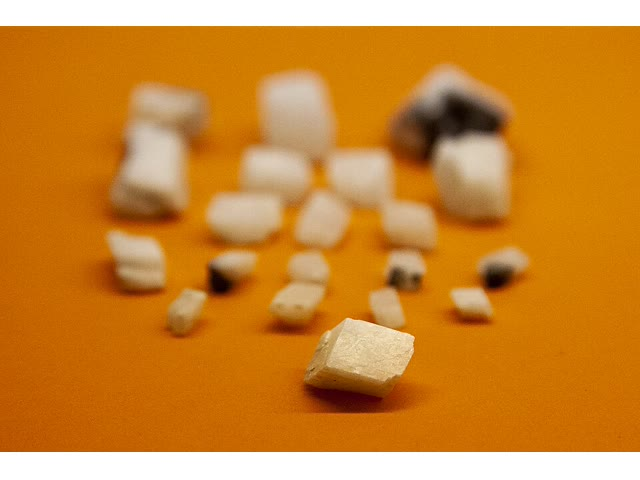
\includegraphics[width=\linewidth]{images/book3/b1-mineral-calcite-rhombs.jpg}

{\scriptsize Romboëders van splijting van calciet. Foto Giovanna Canu en Eva
Santini, CC BY 4.0 (Wikimedia Commons).}
\end{minipage}
\end{inthelab}

\begin{omfigure}
\setlength{\tabcolsep}{2pt}
\begin{tabular}{ccc}
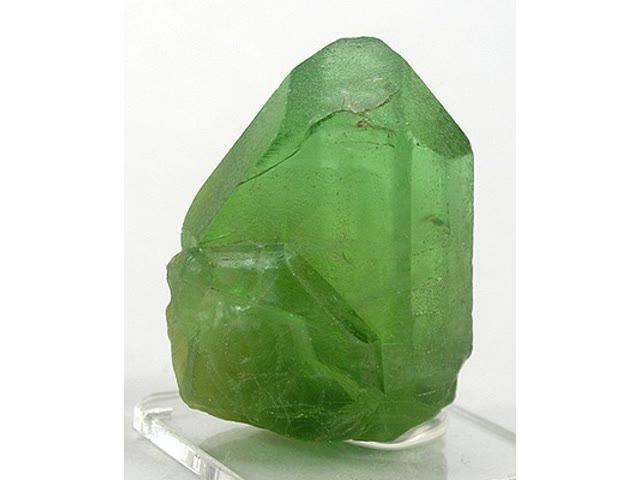
\includegraphics[width=0.31\linewidth]{images/book3/b1-mineral-olivine.jpg} &
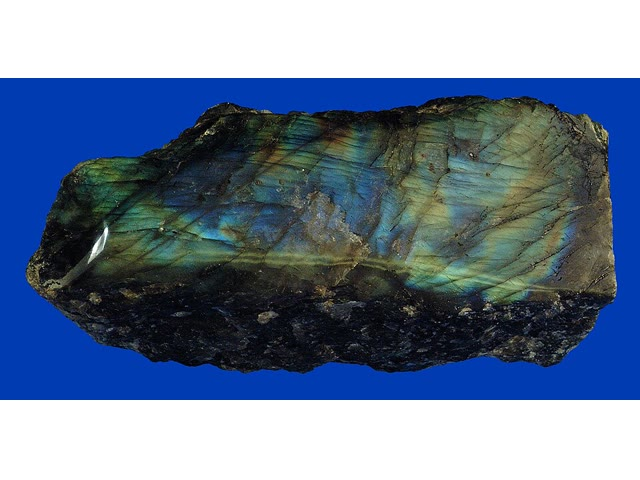
\includegraphics[width=0.31\linewidth]{images/book3/b1-mineral-plagioclase.jpg} &
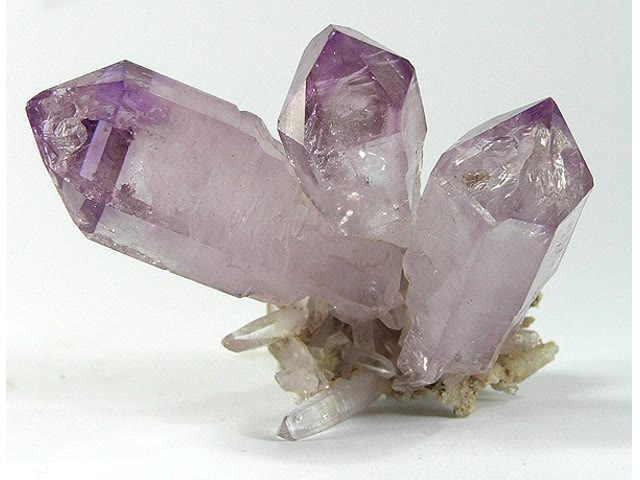
\includegraphics[width=0.31\linewidth]{images/book3/b1-mineral-quartz.jpg} \\
{\small (a) \omterm{def:b1:rock-forming-minerals:groups}{olivijn}} & {\small (b) \omterm{def:b1:rock-forming-minerals:groups}{plagioklaas} (labradoriet)} & {\small (c) kwarts (amethist)} \\[4pt]
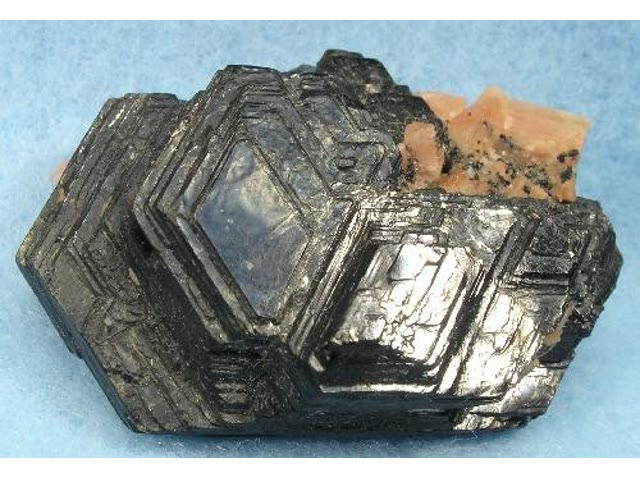
\includegraphics[width=0.31\linewidth]{images/book3/b1-mineral-biotite.jpg} &
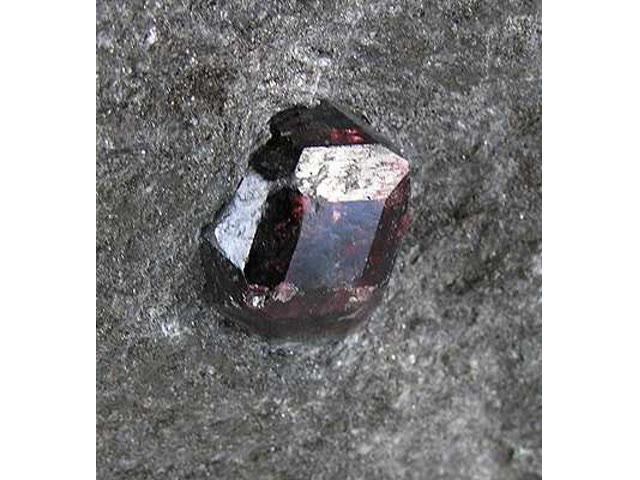
\includegraphics[width=0.31\linewidth]{images/book3/b1-mineral-garnet.jpg} &
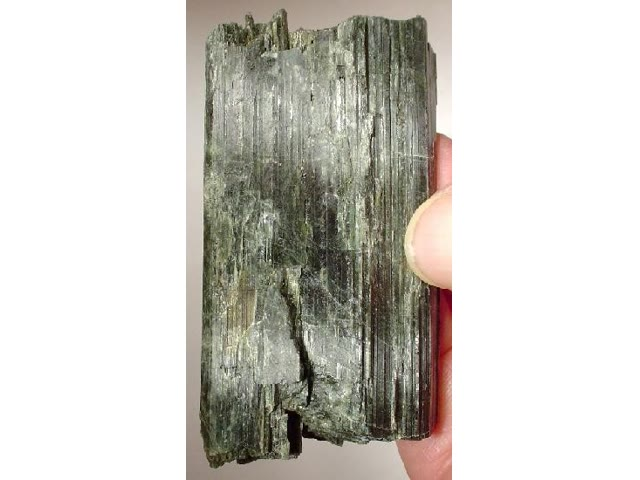
\includegraphics[width=0.31\linewidth]{images/book3/b1-mineral-hornblende.jpg} \\
{\small (d) biotiet op orthoklaas} & {\small (e) \omterm{def:b1:rock-forming-minerals:groups}{granaat} (almandien)} & {\small (f) hoornblende} \\
\end{tabular}
\medskip
% ledger: commons:min-olivine, commons:min-plagioclase, commons:min-quartz, commons:min-biotite, commons:min-garnet, commons:min-hornblende

{\small Zes gesteentevormende mineralen: (a) een edelsteenkristal van \omterm{def:b1:rock-forming-minerals:groups}{olivijn}; (b) een gepolijste plak \omterm{def:b1:rock-forming-minerals:groups}{plagioklaas} die het kleurenspel van
labradoriet toont; (c) kwartskristallen, zeszijdige prisma's met piramidale punten; (d) een boekje van biotietplaatjes op een kristal van
ortoklaas; (e) een almandiengranaatkristal in zijn gesteente; (f) een prisma van hoornblende. Foto's (a), (c)--(f) Robert
M.~Lavinsky, CC BY-SA 3.0; (b) Twyla Baker, CC0 (Wikimedia Commons).}
\end{omfigure}

\section{Oefeningen}

\begin{exercise}[$\star$]\label{exo:b1:rock-forming-minerals:1}
Noem de silicaatklasse van elk anion en geef het aantal $s$ van hoeken dat elk tetraëder deelt: \ce{SiO4^{4-}}, \ce{Si2O7^{6-}},
\ce{Si6O18^{12-}}, \ce{Si2O5^{2-}}, \ce{SiO2}. Tot welke klasse zou \ce{SiO3^{2-}} kunnen behoren?
\end{exercise}

\begin{exercise}[$\star$]\label{exo:b1:rock-forming-minerals:2}
Met de atoomgewichten O \num{15.999}, Si \num{28.085}, Mg \num{24.305} en Fe \qty{55.845}{g.mol^{-1}}, bereken de molaire massa's
van forsteriet en fayaliet, en daarna hun molaire volumes uit de dichtheden \num{3.275} en \qty{4.392}{g.cm^{-3}}.
% ledger: ciaaw:O, ciaaw:Si, ciaaw:Mg, ciaaw:Fe, hom:forsterite, hom:fayalite
\end{exercise}

\begin{exercise}[$\star$]\label{exo:b1:rock-forming-minerals:3}
In zesvoudige coördinatie zijn de stralen \ce{Mg^{2+}} \qty{0.72}{\angstrom}, \ce{Fe^{2+}} \qty{0.78}{\angstrom}, \ce{Ni^{2+}}
\qty{0.69}{\angstrom}, \ce{Mn^{2+}} \qty{0.83}{\angstrom} en \ce{Ca^{2+}} \qty{1.00}{\angstrom}. Bereken het verschil van elk met de straal
van \ce{Mg^{2+}} in procenten, en zeg, volgens de regels van Goldschmidt, welke vrij magnesium in \omterm{def:b1:rock-forming-minerals:groups}{olivijn} kunnen vervangen.
% ledger: shannon:radii, goldschmidt:size
\end{exercise}

\begin{exercise}[$\star$]\label{exo:b1:rock-forming-minerals:4}
Grafiet en diamant hebben dichtheden van \num{2.16} en \qty{3.51}{g.cm^{-3}}; calciet en aragoniet \num{2.71} en \qty{2.93}{g.cm^{-3}}.
Met hoeveel procent stijgt de dichtheid bij elke omzetting? Welke \omterm{def:b1:rock-forming-minerals:polymorph}{polymorf} van elk paar ontstaat bij de hogere druk?
% ledger: webmineral:polymorphs, hom:calcite
\end{exercise}

\begin{exercise}[$\star\star$]\label{exo:b1:rock-forming-minerals:5}
Schrijf de \omterm{def:b1:rock-forming-minerals:formula}{structuurformule} van de \omterm{def:b1:rock-forming-minerals:groups}{plagioklaas} $\text{An}_{30}$ (\qty{30}{\percent} van de grote plaatsen gevuld met calcium), en
controleer dat zij neutraal is.
\end{exercise}

\begin{exercise}[$\star\star$]\label{exo:b1:rock-forming-minerals:6}
In een dubbele keten delen de helft van de tetraëders twee hoeken en de helft drie. Tel de zuurstoffen van een herhalende groep van vier
tetraëders direct op paneel (f) van de koppelingsfiguur, en controleer de formule \ce{Si4O11^{6-}} die door
\cref{prop:b1:rock-forming-minerals:si-o} wordt gegeven.
\end{exercise}

\begin{exercise}[$\star\star$]\label{exo:b1:rock-forming-minerals:7}
Herbereken op vier zuurstoffen de olivijnanalyse \qty{40.20}{\percent} \ce{SiO2}, \qty{47.10}{\percent} \ce{MgO}, \qty{12.20}{\percent} \ce{FeO},
\qty{0.40}{\percent} \ce{NiO} (molaire massa van \ce{NiO} \qty{74.692}{g.mol^{-1}}). Geef haar \omterm{def:b1:rock-forming-minerals:formula}{structuurformule}, controleer die, en geef
haar forsteriet-gehalte. Toon daarna aan dat het forsteriet-gehalte alleen uit de percentages \ce{MgO} en \ce{FeO} kan worden gevonden.
\end{exercise}

\begin{exercise}[$\star\star$]\label{exo:b1:rock-forming-minerals:8}
Controleer dat muscoviet \ce{KAl2(Si3Al)O10(OH)2} neutraal is. Haar lagen van tetraëders hebben één aluminium op drie siliciumatomen: welke
lading geeft dit de laag per formule-eenheid, en welk ion compenseert die?
\end{exercise}

\begin{exercise}[$\star\star$]\label{exo:b1:rock-forming-minerals:9}
Gebruik de molaire volumes \num{42.96} en \qty{46.40}{cm^3.mol^{-1}} en de molaire massa's \num{140.691} en \qty{203.771}{g.mol^{-1}}:
(a) bereken de dichtheid van $\text{Fo}_{50}$ door ideale menging, en vergelijk die met het gemiddelde van de dichtheden van de \omterm{def:b1:rock-forming-minerals:solid-solution}{eindleden};
(b) vind het forsteriet-gehalte van een \omterm{def:b1:rock-forming-minerals:groups}{olivijn} van dichtheid \qty{3.600}{g.cm^{-3}}.
\end{exercise}

\begin{exercise}[$\star\star\star$]\label{exo:b1:rock-forming-minerals:10}
Met de notatie van \cref{prop:b1:rock-forming-minerals:ideal-mixing}, toon aan dat
\[
  \rho(x) - \bigl(x\rho_1 + (1 - x)\rho_2\bigr) =
  \frac{x(1 - x)(\rho_1 - \rho_2)(V_1 - V_2)}{V(x)} .
\]
Leid af dat de dichtheid van \omterm{def:b1:rock-forming-minerals:groups}{olivijn} boven de rechte lijn tussen de \omterm{def:b1:rock-forming-minerals:solid-solution}{eindleden} ligt, en bereken het verschil bij $\text{Fo}_{50}$.
\end{exercise}

\begin{exercise}[$\star\star\star$]\label{exo:b1:rock-forming-minerals:11}
Een \omterm{def:b1:rock-forming-minerals:groups}{plagioklaas} uit een gabbro geeft \qty{54.10}{\percent} \ce{SiO2}, \qty{28.90}{\percent} \ce{Al2O3}, \qty{11.20}{\percent} \ce{CaO},
\qty{5.10}{\percent} \ce{Na2O} en \qty{0.30}{\percent} \ce{K2O} (molaire massa's \num{60.083}, \num{101.961}, \num{56.077}, \num{61.979},
\qty{94.195}{g.mol^{-1}}). Herbereken op acht zuurstoffen; controleer dat de tetraëdrische plaatsen (Si + Al) 4 atomen bevatten en de grote
plaats (Ca + Na + K) 1; controleer de \omterm{def:b1:rock-forming-minerals:substitution}{gekoppelde substitutie} door $\mathrm{Al} - 1$ met Ca te vergelijken; geef het anortietgehalte
$100\,\mathrm{Ca}/(\mathrm{Ca} +
\mathrm{Na} + \mathrm{K})$.
\end{exercise}

\begin{exercise}[$\star\star\star$]\label{exo:b1:rock-forming-minerals:12}
Een microsonde kan \ce{Fe^{2+}} niet van \ce{Fe^{3+}} onderscheiden en meldt al het ijzer als \ce{FeO}. (a) Toon aan dat zuiver magnetiet
\ce{Fe3O4}, op deze manier geanalyseerd, een totaal van \qty{93.09}{\percent} geeft. (b) Herbereken deze analyse op vier zuurstoffen, en
zeg waarom het resultaat onmogelijk is voor een \omterm{def:b1:rock-forming-minerals:mineral}{mineraal} met drie kationen per vier zuurstoffen. (c) Herbereken daarentegen op drie kationen,
en vind de aantallen \ce{Fe^{2+}} en \ce{Fe^{3+}} door te eisen dat de formule neutraal is. (d) Schrijf de analyse opnieuw als \ce{FeO} en
\ce{Fe2O3}, en geef het nieuwe totaal.
\end{exercise}

\section{Probleem: Een olivijn uit een basalt}

\begin{problem}[{Weekendprobleem --- een microsondeanalyse van een olivijn herberekenen, zijn formule schrijven en controleren, en zijn samenstelling,
zijn dichtheid en zijn massa in een kubieke meter basalt bepalen}]
\label{pb:b1:rock-forming-minerals:1}
% invented analysis: figdata/bachelor-1/solid_solution.py (OLIVINE_WT); values: calc/ch07.py
% ledger: ciaaw:O, ciaaw:Si, ciaaw:Mg, ciaaw:Fe, ciaaw:Mn, ciaaw:Ni, ciaaw:Ca, hom:forsterite, hom:fayalite, shannon:radii
De groene kristallen van een basalt zijn \omterm{def:b1:rock-forming-minerals:groups}{olivijn}. Een microsondeanalyse van een van hen geeft, in gewichtsprocenten oxiden:
\begin{center}
\small
\begin{tabular}{lcccccc}
\hline
oxide & \ce{SiO2} & \ce{FeO} & \ce{MnO} & \ce{MgO} & \ce{NiO} & \ce{CaO} \\
gewicht \% & 39.50 & 16.53 & 0.23 & 43.32 & 0.20 & 0.22 \\
\hline
\end{tabular}
\end{center}
De atoomgewichten zijn O \num{15.999}, Si \num{28.085}, Fe \num{55.845}, Mn \num{54.938}, Mg \num{24.305}, Ni \num{58.693}, Ca \qty{40.078}{g.mol^{-1}}.
Forsteriet heeft dichtheid \qty{3.275}{g.cm^{-3}} en fayaliet \qty{4.392}{g.cm^{-3}}.

\medskip
\noindent\textbf{Deel I --- Van oxiden naar kationen.}
\begin{enumerate}
  \item Bereken de molaire massa's van de zes oxiden.
  \item Bereken het totaal van de analyse. Wat had een totaal van \qty{97}{\percent} gesuggereerd?
  \item Bereken het aantal mol van elk oxide in \qty{100}{g} \omterm{def:b1:rock-forming-minerals:groups}{olivijn}.
  \item Bereken de mol zuurstof die zij bevatten, en hun som.
  \item Bereken de mol van elk kation.
  \item Bereken de factor die de zuurstoffen op vier brengt.
  \item Geef het aantal atomen van elk element per vier zuurstoffen, met drie decimalen.
\end{enumerate}

\medskip
\noindent\textbf{Deel II --- De structuurformule.}
\begin{enumerate}[resume]
  \item \omterm{def:b1:rock-forming-minerals:groups}{Olivijn} heeft één tetraëdrische plaats en twee octaëdrische plaatsen per vier zuurstoffen. Bereken de som van de kationen
        behalve silicium, en vergelijk beide plaatstotalen met de ideale formule.
  \item Schrijf de \omterm{def:b1:rock-forming-minerals:formula}{structuurformule} van de \omterm{def:b1:rock-forming-minerals:groups}{olivijn}.
  \item Controleer dat de formule neutraal is, en leg uit waarom deze controle, anders dan die van vraag 8, niet had kunnen mislukken.
  \item Gebruik de ionstralen (\ce{Mg^{2+}} \qty{0.72}{\angstrom}, \ce{Fe^{2+}} \qty{0.78}{\angstrom}, \ce{Ni^{2+}} \qty{0.69}{\angstrom},
        \ce{Mn^{2+}} \qty{0.83}{\angstrom}, \ce{Ca^{2+}} \qty{1.00}{\angstrom}, alle zesvoudig) om uit te leggen waarom nikkel veelvoorkomend
        is in \omterm{def:b1:rock-forming-minerals:groups}{olivijn} en calcium zeldzaam.
  \item De microsonde meldt al het ijzer als \ce{FeO}. Leg uit waarom het totale aantal kationen dat in vraag 7 is gevonden aantoont dat
        de \omterm{def:b1:rock-forming-minerals:groups}{olivijn} geen noemenswaardige \ce{Fe^{3+}} bevat.
\end{enumerate}

\medskip
\noindent\textbf{Deel III --- De samenstelling.}
\begin{enumerate}[resume]
  \item Bereken het forsteriet-gehalte $\mathrm{Fo} = 100\,\mathrm{Mg}/(\mathrm{Mg} +
        \mathrm{Fe})$, op één decimaal.
  \item Wat is het \omterm{def:b1:rock-forming-minerals:formula}{Mg-getal} van de \omterm{def:b1:rock-forming-minerals:groups}{olivijn}? Waarom is het hier gelijk aan het forsteriet-gehalte?
  \item Schrijf de \omterm{def:b1:rock-forming-minerals:groups}{olivijn} als een binaire \omterm{def:b1:rock-forming-minerals:solid-solution}{vaste oplossing} $\mathrm{Fo}_x\mathrm{Fa}_{1-x}$, de Mn, Ni en Ca negerend, en geef het aandeel van zijn
        octaëdrische plaatsen dat ijzer bevat.
  \item Toon aan dat het forsteriet-gehalte kan worden berekend uit de percentages \ce{MgO} en \ce{FeO} alleen, zonder de factor van vraag 6,
        en doe het.
  \item Een \omterm{def:b1:rock-forming-minerals:groups}{olivijn} die later in dezelfde lava is gegroeid, heeft \qty{40.5}{\percent} \ce{MgO} en \qty{20.0}{\percent} \ce{FeO}. Bereken zijn
        forsteriet-gehalte. Welke \omterm{def:b1:rock-forming-minerals:groups}{olivijn} is rijker aan ijzer?
\end{enumerate}

\medskip
\noindent\textbf{Deel IV --- Dichtheid en massa.}
\begin{enumerate}[resume]
  \item Bereken de molaire massa's en de molaire volumes van forsteriet en fayaliet (molaire volumes op twee decimalen).
  \item Neem de \omterm{def:b1:rock-forming-minerals:groups}{olivijn} als de binaire $\mathrm{Fo}_x\mathrm{Fa}_{1-x}$ van vraag 15, met $x$ afgerond op drie decimalen, en bereken
        haar molaire massa en haar molaire volume door ideale menging.
  \item Leid haar dichtheid af, op drie decimalen.
  \item Vergelijk die met de rechte-lijninterpolatie tussen de dichtheden van de \omterm{def:b1:rock-forming-minerals:solid-solution}{eindleden}.
  \item Het basalt bevat \qty{12}{\percent} \omterm{def:b1:rock-forming-minerals:groups}{olivijn} naar volume. Welke massa \omterm{def:b1:rock-forming-minerals:groups}{olivijn} bevat een kubieke meter van het basalt?
  \item Het basalt heeft een dichtheid van \qty{2.95}{g.cm^{-3}}. Wat is het aandeel \omterm{def:b1:rock-forming-minerals:groups}{olivijn} naar massa?
  \item Wat is het forsteriet-gehalte van de \omterm{def:b1:rock-forming-minerals:groups}{olivijn}, afgerond op het hele procent?
\end{enumerate}
\end{problem}
